\subsection{不同模型面数下的 BVH 加速效果}

为验证 BVH 对光线--三角形求交的加速效果，选取四个不同面数的 Stanford 模型对比实验。分辨率均为
$1280\times960$、\texttt{spp}=1，渲染内容与光照一致，仅替换输入网格。对每个模型测试两种模式：启用 BVH 的
正常渲染，以及关闭 BVH、逐三角形暴力遍历的 \texttt{check} 模式（经 \texttt{getIntersectionNoBVH} 绕过网格
内部 BVH、直接遍历全部三角形）。整个流程由脚本 \texttt{run\_experiments\_ubuntu.sh} 在 Release（\texttt{-O3}）
构建下完成，\textbf{两种模式使用相同的 32 线程（OpenMP）}以保证同硬件、同并行度下的公平对照；脚本解析
\texttt{Render seconds} 并汇总为 \texttt{summary.csv}，同时对每个模型 BVH 与 check 输出做 \texttt{cmp} 字节级
核对，四个模型均\textbf{逐像素一致}。结果如表~\ref{tab:bvh-speedup-models}、图~\ref{fig:speedup} 与
图~\ref{fig:bvh-models} 所示。

\begin{table}[htbp]
  \centering
  \caption{不同模型面数下 BVH 与暴力求交渲染时间对比（同 32 线程，\texttt{spp}=1）}
  \label{tab:bvh-speedup-models}
  \begin{tabular}{lrrrrr}
    \hline
    模型 & 顶点数 & 面数 & BVH 渲染时间/s & 无 BVH 渲染时间/s & 加速比 \\
    \hline
    Bunny       & 2503   & 4968   & 0.0404 & 1.450   & 35.89   \\
    Dragon res3 & 22998  & 47794  & 0.0420 & 30.529  & 726.44  \\
    Dragon res2 & 100250 & 202520 & 0.0495 & 139.352 & 2813.15 \\
    Armadillo   & 172974 & 345944 & 0.0344 & 226.813 & 6588.31 \\
    \hline
  \end{tabular}
\end{table}

\begin{figure}[htbp]
  \centering
  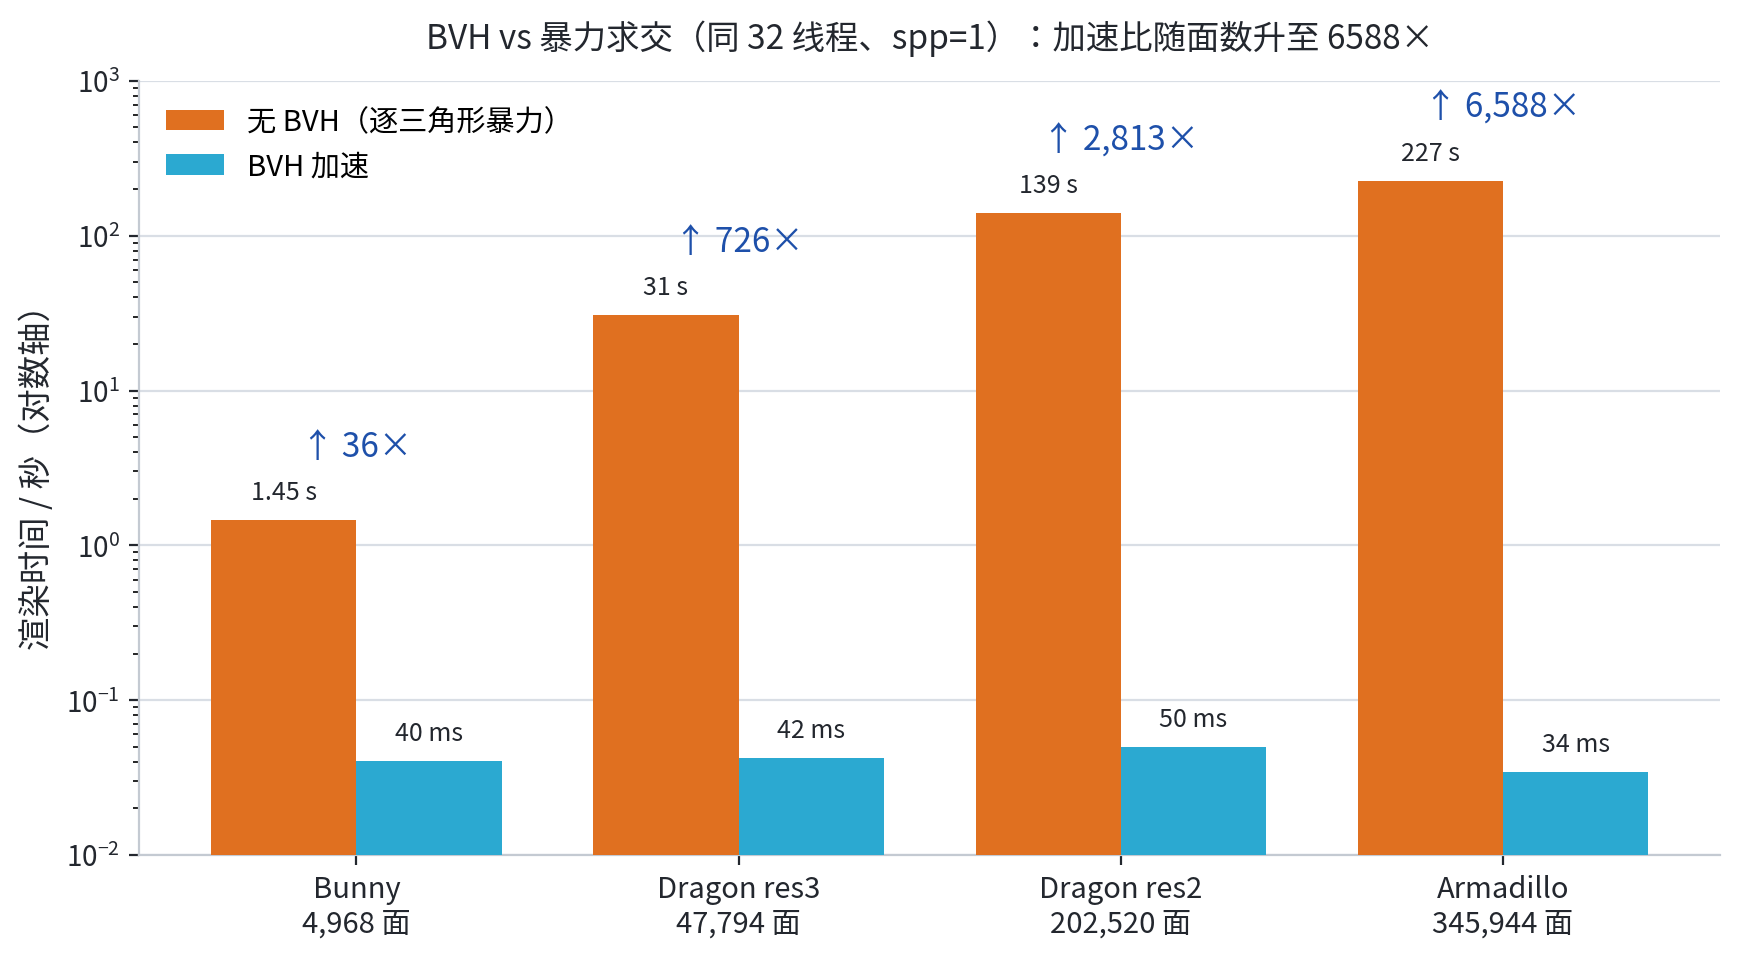
\includegraphics[width=0.92\textwidth]{figures/speedup.png}
  \caption{BVH 与逐三角形暴力求交的渲染时间对比（对数轴，同 32 线程）。暴力求交时间随面数从
  $1.45\,\mathrm{s}$ 增长到 $226.8\,\mathrm{s}$，而 BVH 始终保持在数十毫秒量级；加速比从 $36$ 倍升至 $6588$ 倍。}
  \label{fig:speedup}
\end{figure}

\begin{figure}[htbp]
  \centering
  \begin{subfigure}{0.32\textwidth}
    \centering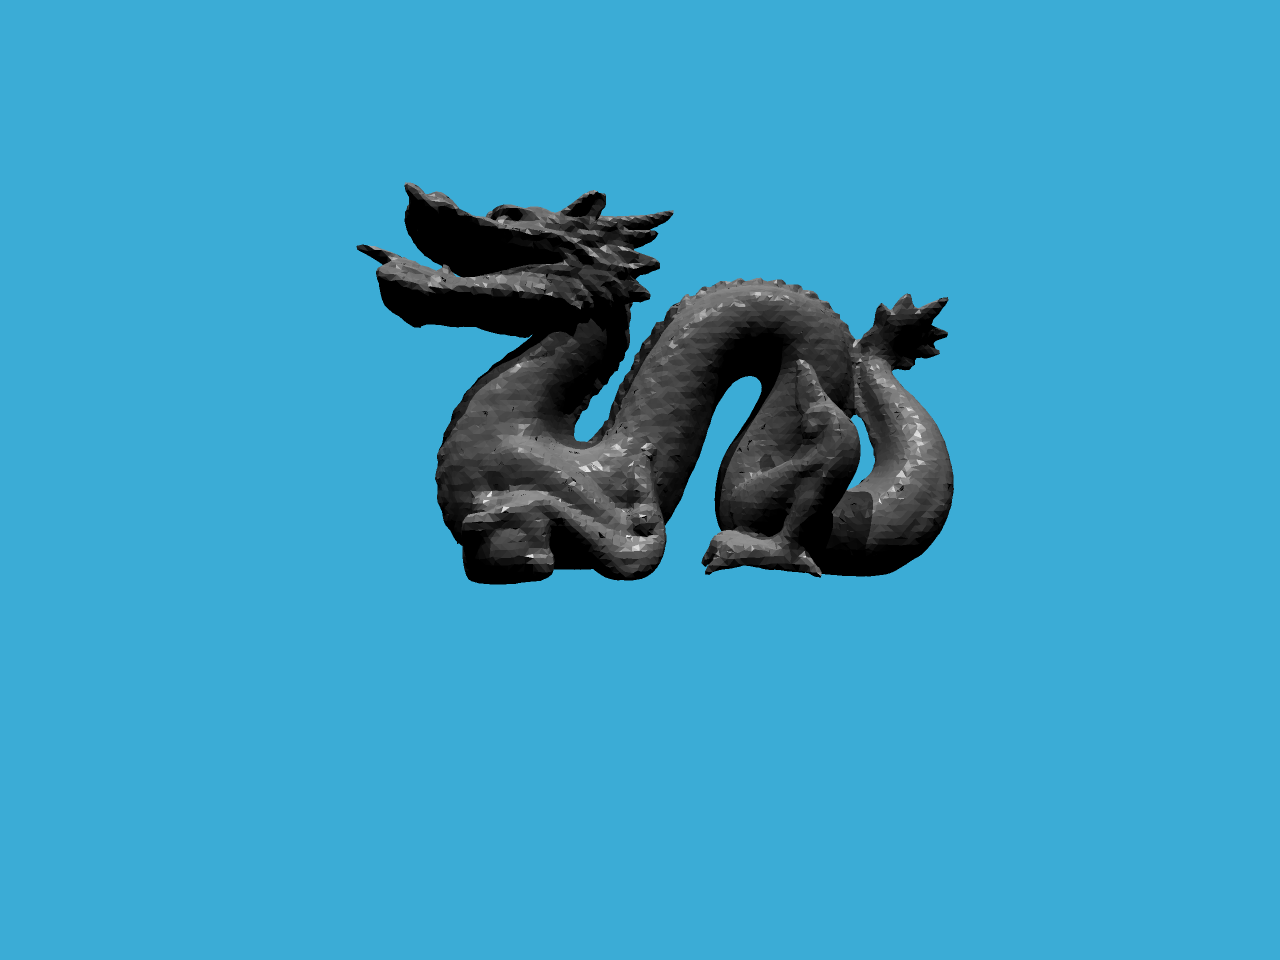
\includegraphics[width=\textwidth]{figures/dragon_res3_bvh.png}
    \caption{Dragon res3（47794 面）}
  \end{subfigure}\hfill
  \begin{subfigure}{0.32\textwidth}
    \centering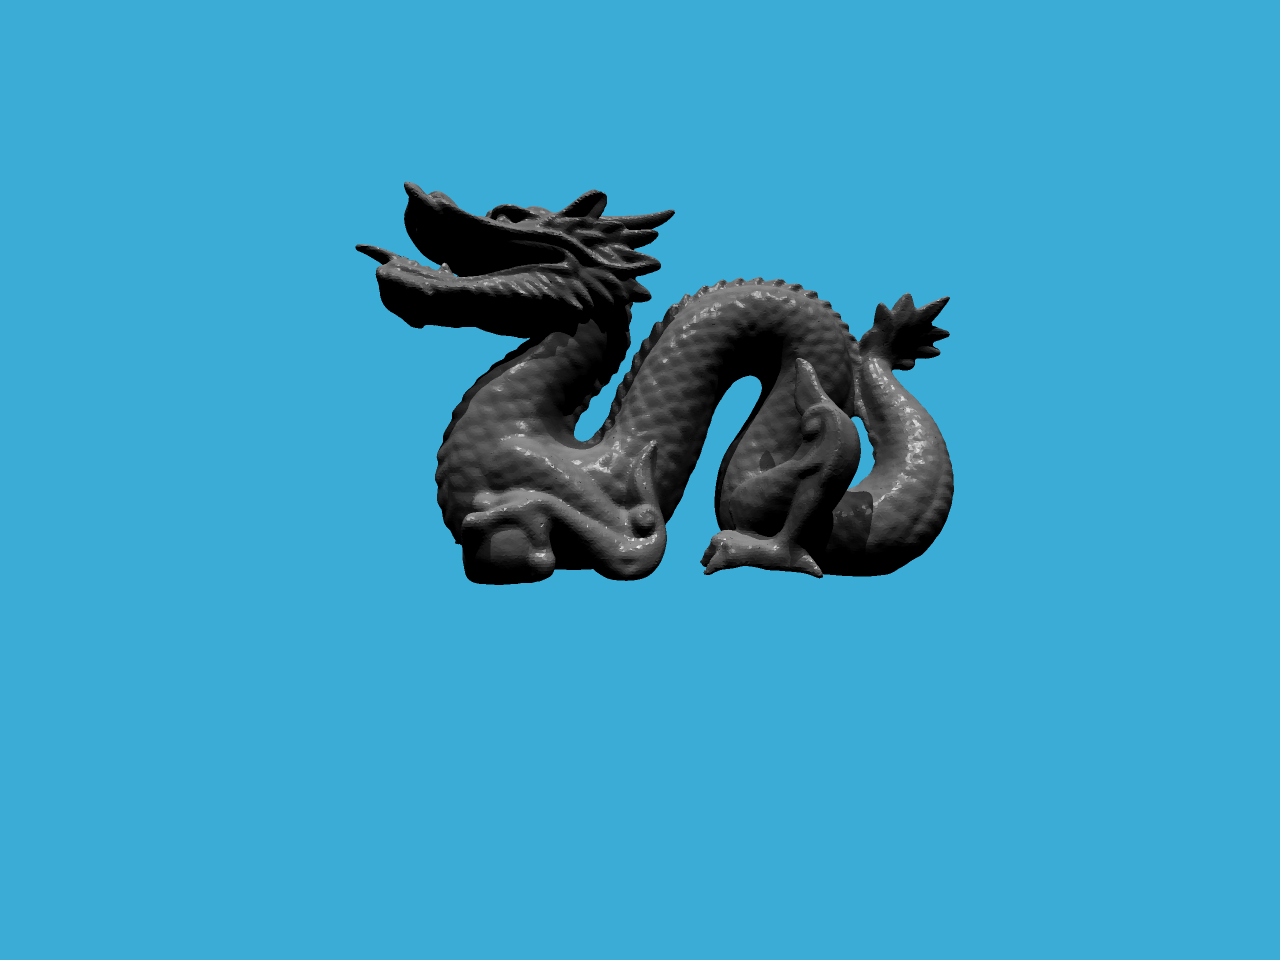
\includegraphics[width=\textwidth]{figures/dragon_res2_bvh.png}
    \caption{Dragon res2（202520 面）}
  \end{subfigure}\hfill
  \begin{subfigure}{0.32\textwidth}
    \centering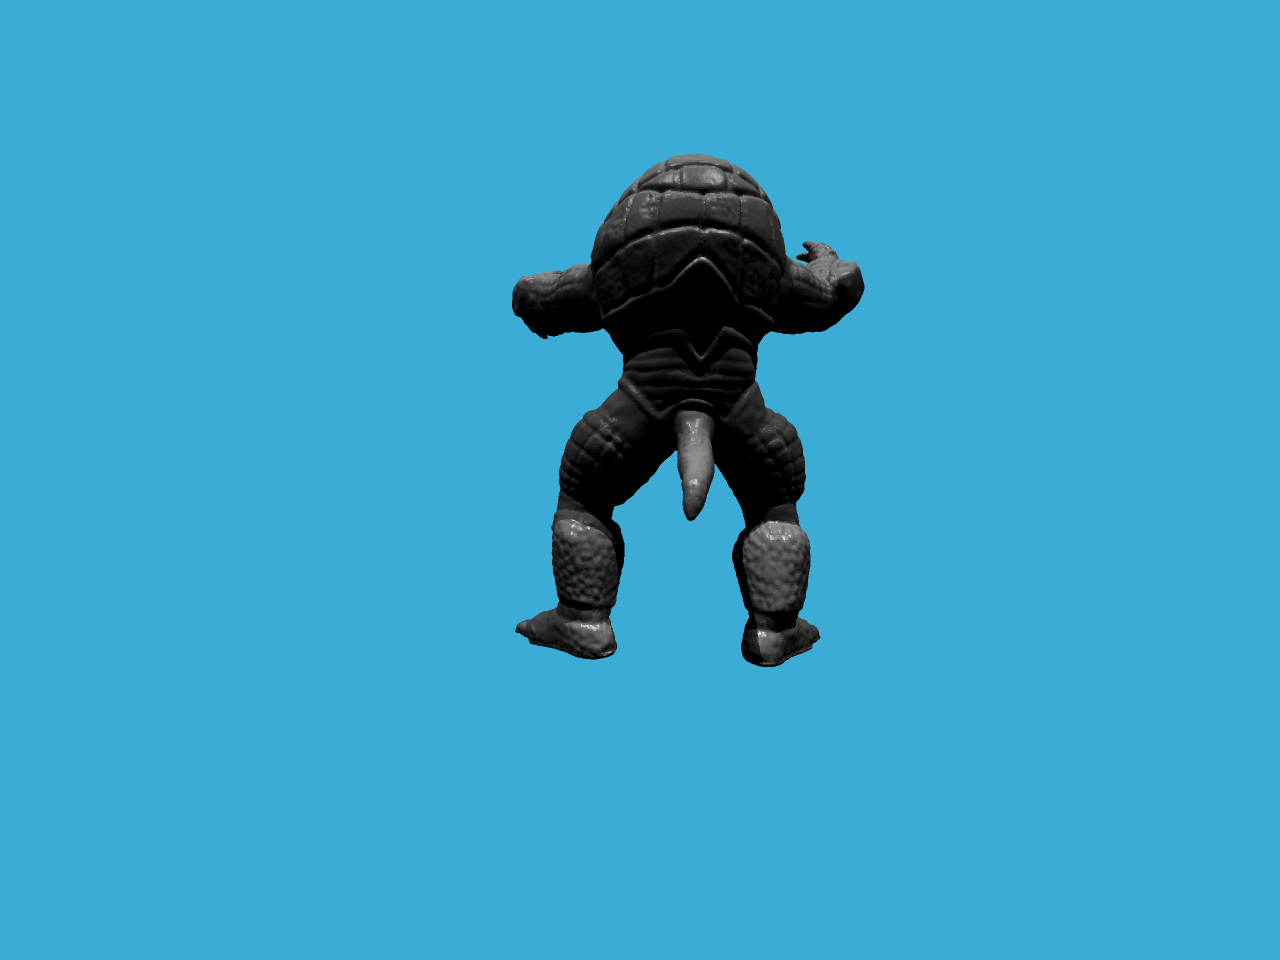
\includegraphics[width=\textwidth]{figures/armadillo_bvh.png}
    \caption{Armadillo（345944 面）}
  \end{subfigure}
  \caption{三个不同面数 Stanford 模型在 BVH 模式下的渲染结果（$1280\times960$、\texttt{spp}=2 抗锯齿）。
  三幅图像均带有正确的漫反射、\textbf{镜面高光}与自阴影；随面数增加表面细节愈发丰富，而 BVH 渲染耗时仍稳定在数十毫秒。}
  \label{fig:bvh-models}
\end{figure}

从实验结果可以看出，BVH 对三角网格渲染具有非常显著的加速效果。在同样的 32 线程下，面数最少的 Bunny（$4968$ 面）
暴力求交需 $1.45\,\mathrm{s}$、BVH 仅 $40\,\mathrm{ms}$（$36$ 倍）；Armadillo（$345944$ 面）暴力求交达
$226.8\,\mathrm{s}$、约 $3.8$ 分钟，而 BVH 仍能在 $34\,\mathrm{ms}$ 内完成，加速比高达 $6588$ 倍。
其根本原因在于：暴力求交对每条光线都要遍历模型全部三角形，计算量随面数近似线性增长（$1280\times960$ 下主光线
已超百万条，叠加阴影光线后求交次数更多）；而 BVH 先用廉价的包围盒测试剪掉大片不可能相交的空间，单条光线实际
访问的三角形数量大幅减少，故 BVH 时间几乎不随面数增长。需要说明的是，由于本次两种模式都已多线程并行，暴力基线
不再是分钟至小时级，而是秒级，因此这里的加速比（$36$--$6588$ 倍）低于早期单线程版本的数字，但二者仍处于同一
硬件、同一并行度下，是\textbf{公平的同条件对照}。

\subsection{BVH 随面数的缩放与多线程加速}

为更清晰地展示 BVH 的缩放特性，进一步测量\textbf{单线程}下 BVH 随面数的渲染时间，以及 Bunny 在不同线程数下的
加速曲线（均 \texttt{spp}=1），如图~\ref{fig:scaling} 所示，原始数据见 \texttt{bvh\_scaling.csv}、
\texttt{thread\_scaling.csv}。

\begin{figure}[htbp]
  \centering
  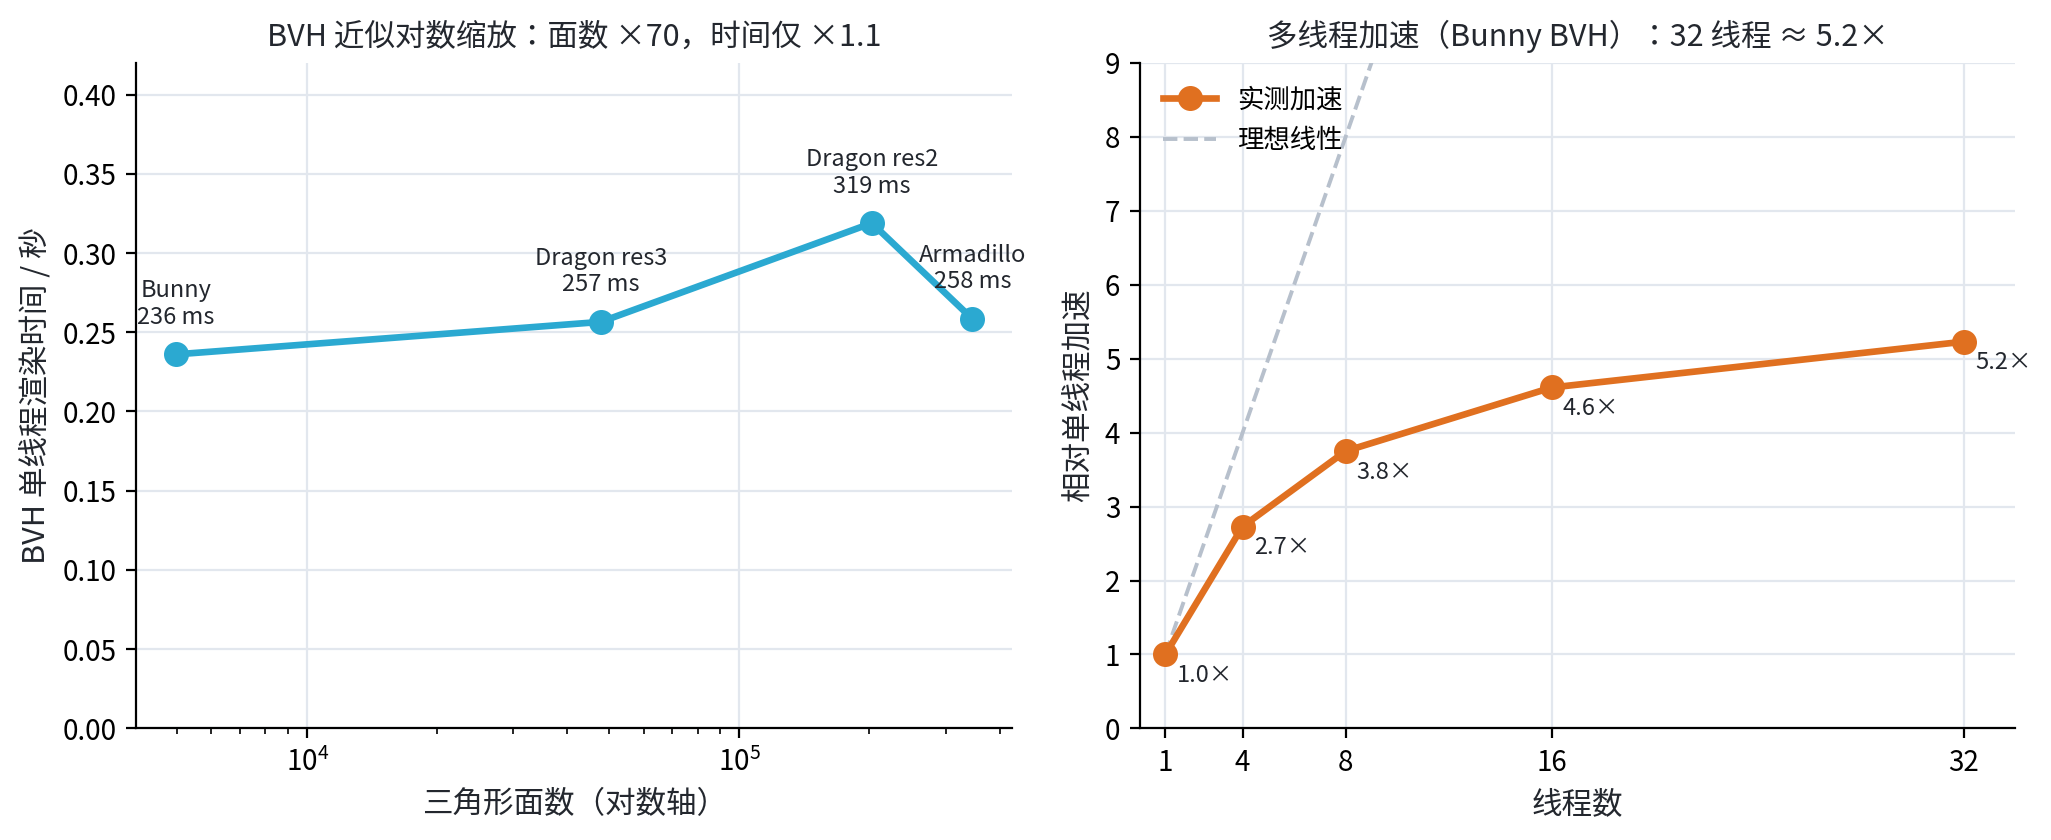
\includegraphics[width=0.95\textwidth]{figures/scaling.png}
  \caption{左：单线程 BVH 渲染时间随面数的变化——面数从 $4968$ 增至 $345944$（约 $\times70$），BVH 时间仅从
  $236\,\mathrm{ms}$ 变到 $258\,\mathrm{ms}$（约 $\times1.1$），近似对数缩放；右：Bunny BVH 的多线程加速曲线，
  $32$ 线程相对单线程约 $5.2$ 倍（小负载下受固定开销与 Amdahl 限制，加速未达线性，重负载场景可更高）。}
  \label{fig:scaling}
\end{figure}

左图证实了 BVH 的核心优势：模型复杂度提升约 $70$ 倍，单线程 BVH 渲染时间几乎不变，体现出对数级而非线性的
求交复杂度。右图表明，在本文新增的 OpenMP 并行下，渲染可进一步获得数倍加速；Bunny 这类亚秒级小负载因固定开销
占比较高、加速曲线趋于平缓（$32$ 线程约 $5.2$ 倍），而暴力基线这类秒级以上的重负载并行效率更高。

综上，BVH（求交算法层面）与多线程（并行层面）是两个正交的加速来源：前者把同场景的渲染时间从分钟级压到毫秒级、
且几乎不随面数增长，后者在此之上再叠加数倍加速。两者共同使复杂网格的光线追踪渲染达到实用速度。
